\documentclass[xcolor=x11names,compress,professionalfonts, aspectratio=169]{beamer}

%% General packages %%%%%%%%%%%%%%%%%%%%%%%%%%%%%%%%%%
\usepackage[utf8]{inputenc}
\usepackage{graphicx}
\usepackage{tikz}
\tikzset{% change default arrow tips
    >=latex
}
\usepackage{ifthen}

\usepackage{nicefrac}

\usepackage{color}
\usepackage[french]{babel} %français
\usepackage{amsmath, amssymb, amsfonts, mathtools}
\usepackage{physics}
\usepackage{forloop}
\usepackage[makeroom]{cancel}

%%%%%%%%%%%%%%%%%%%%%%%%%%%%%%%%%%%%%%%%%%%%%%%%%%%%%%

\makeatletter
\setbeamertemplate{footline}
{
    \leavevmode%
    \hbox{%
        \begin{beamercolorbox}[wd=.333333\paperwidth,ht=2.25ex,dp=1ex,center]{author in head/foot}%
            \usebeamerfont{author in head/foot}\insertshortauthor
        \end{beamercolorbox}%
                \begin{beamercolorbox}[wd=.333333\paperwidth,ht=2.25ex,dp=1ex,center]{title in head/foot}%
            \usebeamerfont{title in head/foot}\insertshorttitle
        \end{beamercolorbox}%
        \begin{beamercolorbox}[wd=.333333\paperwidth,ht=2.25ex,dp=1ex,right]{date in head/foot}%
            \usebeamerfont{date in head/foot}\insertshortdate{}\hspace*{2em}
            \insertframenumber{} / \inserttotalframenumber\hspace*{2ex} 
        \end{beamercolorbox}}%
        \vskip0pt%
    }
    \makeatother


%% Beamer Layout %%%%%%%%%%%%%%%%%%%%%%%%%%%%%%%%%%
\useoutertheme[subsection=false,shadow]{miniframes}
\useinnertheme{rectangles}

\setbeamertemplate{navigation symbols}{}%remove navigation symbols

\author{Nicolas Macé}

\newcommand{\btVFill}{\vskip0pt plus 1filll}%place an element at the bottom of the page

\usepackage{libertine}
\usepackage[T1]{fontenc}

\setbeamerfont{title like}{shape=\scshape}
\setbeamerfont{frametitle}{shape=\scshape}

\setbeamercolor*{lower separation line head}{bg=DeepSkyBlue4} 
\setbeamercolor*{normal text}{fg=black,bg=white} 
\setbeamercolor*{alerted text}{fg=red} 
\setbeamercolor*{example text}{fg=black} 
\setbeamercolor*{structure}{fg=black} 
 
\setbeamercolor*{palette tertiary}{fg=black,bg=black!10} 
\setbeamercolor*{palette quaternary}{fg=black,bg=black!10} 

\renewcommand{\(}{\begin{columns}}
\renewcommand{\)}{\end{columns}}
\newcommand{\<}[1]{\begin{column}{#1}}
\renewcommand{\>}{\end{column}}

% custom commands and definitions
%------------------ General setup ------------------%
\definecolor{darkblue}{rgb}{0.0,0.0,0.4}
\hypersetup
{
bookmarksopen=true,
pdftitle=Nicolas Macé - Electronic properties of quasicrytals,
pdfauthor=Nicolas Macé, 
pdfsubject=Electronic properties of quasicrytals, %subject of the document
%pdftoolbar=false, % toolbar hidden
pdfmenubar=true, %menubar shown
pdfhighlight=/O, %effect of clicking on a link
colorlinks=true, %couleurs sur les liens hypertextes
pdfpagemode=None, %aucun mode de page
pdfpagelayout=SinglePage, %ouverture en simple page
pdffitwindow=true, %pages ouvertes entierement dans toute la fenetre
linkcolor=darkblue, %couleur des liens hypertextes internes
citecolor=RoyalBlue, %couleur des liens pour les citations
urlcolor=darkblue %couleur des liens pour les url
}

%---------------- Commands ---------------------------%

%%%%%%%%%%%%%% TYPOGRAPHY %%%%%%%%%%%%%%%%%%%%%%%%%%%%%

% id est
\newcommand{\ie}{i.e.}
% eg
\newcommand{\eg}{e.g.}

%%%%%%%%%%%%%% MISC %%%%%%%%%%%%%%%%%%%%%%%%%%%%%%%%%%%%%

% et al
\newcommand{\etal}{\textit{et~al.}\xspace}
% vector notation
\renewcommand{\vec}[1]{\mathbf{#1}}
% the equal sign I use to define something
\newcommand{\define}{\ensuremath{ \overset{\text{def}}{=} }}
% card sine
\DeclareMathOperator{\sinc}{sinc}
% differential element
\renewcommand{\d}[1]{\mathrm{d}#1}
% similar symbol with a limit underneath
\newcommand{\simlim}[1]{\ensuremath{ \underset{#1}{\sim} }}
% alias for omega
\newcommand{\om}{\ensuremath{\omega}}
% local part of the KK wavefunction
\DeclareMathOperator{\loc}{C}
% idos
\newcommand{\idos}{\ensuremath{\text{idos}}}
% hermitian conjugate
\newcommand{\hc}{\ensuremath{\text{H.c}}}
% region on the tiling
\newcommand{\reg}{\ensuremath{\mathcal{R}}}
% generating function of the height stat
\newcommand{\gen}{\ensuremath{Z}}
% volume of a region
\newcommand{\vol}{\ensuremath{\text{Vol}}}
% Ammann-Beenker alias
\newcommand{\AB}{Ammann-Beenker}
% SKK alias
\newcommand{\SKK}{SKK}
% sim symbol with a limit underneath
\newcommand{\simop}[1]{\ensuremath{\underset{#1}{\sim}}}

% differential element
\renewcommand{\d}[1]{\mathrm{d}#1}

\newcommand{\lb}{\ensuremath{\overline{\lambda}}}
\newcommand{\zb}{\ensuremath{\overline{z}}}
% wavefunction dimensions
\newcommand{\wf}{\ensuremath{d^\psi}}
% averaged wavefunction dimensions
\newcommand{\avwf}{\ensuremath{\overline{D^\psi}}}
% local spectral dimensions
\newcommand{\locspec}{\ensuremath{D^\mu}}
% averaged local spectral dimensions
\newcommand{\avspec}{\ensuremath{D^\mu}}
% bold g letter in math mode
\newcommand{\gv}{\ensuremath{\mathbf{g}}}

% log derivative of the wavefunction
\newcommand{\dlogpsi}{\ensuremath{\d \log \psi}}
% average potential
\newcommand{\meanv}{\ensuremath{\langle V \rangle}}
% ceiling function
\DeclarePairedDelimiter{\ceil}{\lceil}{\rceil}
% floor function
\DeclarePairedDelimiter{\floor}{\lfloor}{\rfloor}
% irrational number
\newcommand{\irr}{\ensuremath{\alpha}}
% cut-and-project
\renewcommand{\cp}{C\&P}
% set of the integers
\newcommand{\zahl}{\ensuremath{\mathds{Z}}}
% fractional part function
\DeclarePairedDelimiter{\fpart}{\{}{\}}
% normalized perp position
\newcommand{\nperp}[2]%
	{%
		\ifthenelse{\isempty{#1}}{\ensuremath{\widetilde{x}_\perp}}{\ensuremath{\widetilde{x}_\perp(#1,#2)}}%
	}
% average with angled brackets
\DeclarePairedDelimiter{\avg}{\langle}{\rangle}
% sturmian fucntion (generate a sturmian sequence)
\newcommand{\sturm}[2]{\ensuremath{S_{#1}\left(#2\right)}}
% Heaviside function
\DeclareMathOperator{\heaviside}{Y}
% support of the multifractal spectrum
\newcommand{\supp}{\ensuremath{\Delta_f}}
% variational groundstate
\newcommand{\psivar}{\ensuremath{\psi_\text{var}}}
% preexponential factor for the variational groundstate
\newcommand{\locvar}{\ensuremath{C_\text{var}}}

%%%%%%%%%%%%%%%%% COMMENTS %%%%%%%%%%%%%%%%%%%%%%%%%%%
\newcommand{\nico}[1]{\textcolor{BrickRed}{#1}}
\newcommand{\anu}[1]{\textcolor{NavyBlue}{#1}}
\newcommand{\fred}[1]{\textcolor{OliveGreen}{#1}}

%%%%%%%%%%%%%%%% QUANTUM MECHANICS %%%%%%%%%%%%%%%%%
% energy
\newcommand{\en}{\ensuremath{\varepsilon}}
% Operator
\renewcommand{\op}[1]{\hat{#1}}
% density of states
\DeclareMathOperator{\dos}{\rho}

%%%%%%%%%%%%%%%% ALPHABETS AND WORDS %%%%%%%%%%%
% the A letter
\newcommand{\A}{\ensuremath{\text{A}}}
% the B letter
\newcommand{\B}{\ensuremath{\text{B}}}
% any sequence of letters
\newcommand{\lett}[1]{\ensuremath{\text{#1}}}
% letter couting function: #1 is the word we count in, #2 is the sequence of letters counted
\newcommand{\nb}[2]{\ensuremath{|#1|_{#2}}}
% substitution
\DeclareMathOperator{\sub}{S}
% word (infinite)
\newcommand{\word}{\ensuremath{w}}
% word complexity
\newcommand{\cmplx}[2]%
	{%
		\ifthenelse{\isempty{#1}}{\ensuremath{\Omega}}{\ensuremath{\Omega(#1,#2)}}%
	}

%%%%%%%%%%%%%%% PERIODIC CRYSTALS %%%%%%%%%%%%%%
\newcommand{\kvec}{\ensuremath{\mathbf{k}}}

%%%%%%%%%%%%%%% MULTIFRACTAL ANALYSIS %%%%%%%%%%
\newcommand{\bc}{box-counting}
% mass (or probability measure) defining a fractal set
\DeclareMathOperator{\mass}{\mu}
% q weight
\DeclareMathOperator{\qweight}{\text{M}}
% partition into a set of boxes
\DeclareMathOperator{\boxset}{\mathcal{B}}
% pointwise Hölder exponent
\DeclareMathOperator{\hold}{\alpha}



\begin{document}

\begin{frame}
\title{Thermalization and localization in one-dimensional quantum systems}

\author{Nicolas Macé}

\date{Janurary 30, 2019}

\titlepage

\btVFill
\begin{columns}
\begin{column}{2cm}
~\\
~\\
~\\
~\\
\raggedright
\includegraphics[scale=.15]{img/title/logo-ups.png}
\end{column}
\begin{column}{6cm}
\centering
\includegraphics[width=.8\textwidth]{img/title/cover.png}
\end{column}
\begin{column}{2cm}
~\\
~\\
~\\
~\\
\raggedleft
\includegraphics[scale=.15]{img/title/LPT-LOGO_RVB.jpg}
\end{column}
\end{columns}
\end{frame}

\section*{Parcours}
\subsection{Dummy}
\begin{frame}{Parcours}
\begin{block}{}
Cursus universitaire (M2 de physique théorique, Paris)
\end{block}
%
\begin{block}{}
(2014-17) \textbf{Doctorat}, dir.\ Anuradha Jagannathan, LPS, Orsay.

\emph{Électrons multifractals en 1D et 2D, Atomes froids quasipériodiques.}
\end{block}
%
\begin{block}{}
(2017-19) \textbf{Postdoctorat}, Nicolas Laflorencie \& Fabien Alet, LPT, Toulouse.

\emph{Localisation à $N$ corps et quasipériodicité, Multifractalité, Méthodes numériques.}
\end{block}
\end{frame}

%\begin{frame}{Plan}
%\tableofcontents[hideallsubsections]
%\end{frame}
\section{Travaux}
\subsection{Dummy}
\begin{frame}{Doctorat : multifractalité dans les quasicristaux}
\centering
Pavage quasipériodique :
~\\
~\\
\only<1>
{
\includegraphics[height=0.6\textheight]{img/1_travaux/no_overlap}

\phantom{presque périodique}

\phantom{Physique : alliages métalliques, atomes froids, bicouche de graphène}
}
\only<2>
{
\includegraphics[height=0.6\textheight]{img/1_travaux/overlap}

$\to$ presque périodes

Physique : alliages métalliques, atomes froids, bicouche de graphène
}
\end{frame}

\begin{frame}{Doctorat : multifractalité dans les quasicristaux}
\textbf{Motivation} : fonctions d'ondes \textbf{fractales}, physique \textbf{critique}

~

\begin{columns}
	\begin{column}{0.5\textwidth}
		1D : Chaîne de Fibonacci 
		
		{
		\centering
		\documentclass[../talk.tex]{subfiles}
\begin{document}


    	\begin{tikzpicture}[scale=.7]
    		\newcommand{\orig}{-1.5}
    		\newcommand{\trans}{1.5}
    		\newcommand{\vertspac}{-2.}
    		\newcommand{\vertsize}{0} % vertical span of the rectangles
    		\newcommand{\del}{.2}
    		\newcommand{\rad}{2pt} % radii of the circles

    		
    		% set the style of the strong bonds
    		\tikzset{
    			strong/.style={
    				double,
    				double distance=\rad,
    				line width=0.5pt
    				}
    		}
    	
    		% initial chain
    	
    		% bonds 
        	\draw[-] (\orig, 0)  node [left] {...}  -- (\orig+\trans, 0) node [midway, below] {$t_w$};
			\draw[strong] (\orig+\trans,0) -- (\orig+2*\trans,0) node [midway, below] {$t_s$};
			\draw[-] (\orig+2*\trans,0) -- (\orig+3*\trans,0) node [midway, below] {$t_w$};	
			\draw[strong] (\orig+3*\trans,0) -- (\orig+4*\trans,0) node [midway, below] {$t_s$};
			\draw[-] (\orig+4*\trans,0) -- (\orig+5*\trans,0) node [midway, below] {$t_w$};
			\draw[-] (\orig+5*\trans,0) -- (\orig+6*\trans,0) node [midway, below] {$t_w$};
			\draw[strong] (\orig+6*\trans,0) -- (\orig+7*\trans,0) node [midway, below] {$t_s$};
			\draw[-] (\orig+7*\trans,0) -- (\orig+8*\trans,0) node [right] {...} node [midway, below] {$t_w$};
    	
    		% sites
			\foreach \x in {0,...,8}
		      \filldraw (\orig+\x*\trans,0) circle (\rad); % node [below] {$\ket{\x}$};
		     
		    

		\end{tikzpicture}

\end{document}
		%
		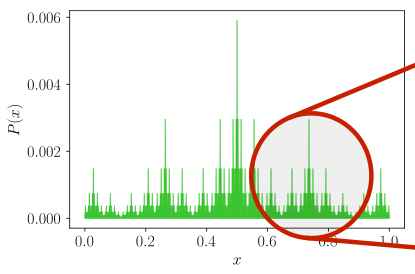
\includegraphics[width=\columnwidth]{img/1_travaux/heights}
		}
	\end{column}
	\begin{column}{0.5\textwidth}
		2D : Pavage octogonal
		\includegraphics[width=\columnwidth]{img/1_travaux/SKK}
	\end{column}
\end{columns}
\textbf{Méthodes} : groupe de renormalisation perturbatif, calcul variationnel (PRB 2016, 2017).
\end{frame}

\begin{frame}{Dimensions multifractales}
Dimensions fractales \textbf{exactes}, modèles \textbf{génériques} (PRB 2017)

\hfill {\footnotesize[Sutherland 86, Repetowicz \emph{et al} 98, Kalugin Katz 14]}

\begin{columns}
	\begin{column}{0.5\textwidth}
		\begin{align*}
			D_q(\lambda) &= \frac{q \theta(\lambda) - \theta(\lambda^q))}{(q-1)\theta(1)} \\
			\theta_{1D}(\lambda) &= \arcsin\left(\frac{(\lambda + \lambda^{-1})^2}{2}\right) \\
			\theta_{2D}(\lambda) &= \arccos(4\lambda + 9 + 4\lambda^{-1})
		\end{align*}
	\end{column}
	\begin{column}{0.5\textwidth}
		Transport \textbf{anormal}
		\centering
		\includegraphics[width=0.9\columnwidth]{img/1_travaux/transport}
	\end{column}
\end{columns}

\textbf{Perspectives} : topologie, robustesse (désordre, interactions).
\end{frame}

\begin{frame}{Postdoc : interactions, localisation à $N$ corps}
\begin{block}{\textbf{Dynamique quantique}, en présence d'\textbf{interactions fortes} et de \textbf{désordre}}
	\begin{enumerate}
		\item Générique :  \textcolor{comp}{thermalisation, décohérence rapide},
		\item Inhabituel : \textcolor{BostonBlue}{non-ergodicité, cohérence longue, \textbf{localisation à $N$ corps}}.
	\end{enumerate}
\end{block}

\begin{columns}
\begin{column}{0.5\textwidth}
\centering
\includegraphics[width=0.9\columnwidth]{img/1_travaux/Imbalance_Choi_thermal}

\includegraphics[width=0.9\columnwidth]{img/1_travaux/Imbalance_Choi}

[Choi \emph{et al} 16]
\end{column}
\begin{column}{0.5\textwidth}
\textbf{Expériences} : atomes/ions froids. Films supraconducteurs ?

\textbf{Motivations} : transition de phase thermal-localisé, nature phase localisée

\textbf{Méthodes} : diagonalisation exacte

taille record $L=26$ (SciPost 2018)
\end{column}
\end{columns}
\end{frame}

\begin{frame}{Postdoc : un modèle de la localisation à $N$ corps}
Fermions en interaction :
\[
	H = \sum_{i=1}^L \left[ J (c_i^\dagger c_{i+1} + \text{h.c}) + \Delta n_i n_{i+1} - h_i n_i \right]
\]

{
\centering
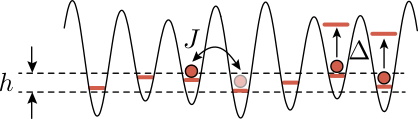
\includegraphics[width=0.5\textwidth]{img/1_travaux/XXZ_cold_atoms}

}
Modèle générique : décrit fermions, spins, bosons de cœur dur.

Désordre : pilote la transition de phase :

{
\centering

\includegraphics[width=0.5\textwidth]{img/1_travaux/arrow}

}
\end{frame}

\begin{frame}{Postdoc : localisation à $N$ corps \& multifractalité}
\begin{columns}
	\begin{column}{0.5\textwidth}
		États propres dans la phase localisée ?
	
		\textbf{Multifractalité} dans l'espace de Hilbert (arxiv 2018)
		
		Espace de Hilbert : graphe complexe, $\text{Vol} \sim 2^L/\sqrt{L}$
		
		\centering		
		\includegraphics[width=0.6\columnwidth]{img/1_travaux/graph_L_6}
	\end{column}
	\begin{column}{0.5\textwidth}
		{		
		\centering
		\includegraphics[width=0.8\columnwidth]{img/1_travaux/scalings}
		
		}		
		Analyse d'échelle : sonde les phases thermales et localisées et leur transition
				
	\end{column}
\end{columns}
\textbf{Perspectives} : nature phase thermale, localisation en 2D, conditions non-thermalisation
\end{frame}
\section{Projet de recherche}
\subsection{Dummy}

\begin{frame}{Cohérence et thermalisation dans les systèmes en interaction}
\textbf{Objectifs} : ingénierie de systèmes robustement cohérents, compréhension du couplage à l'environnement et thermalisation.

\textbf{Contexte grenoblois} : manipulation de qubits (institut Néel, CEA), théorie des systèmes quantiques (LPMMC, institut Néel, CEA, LIG).

\begin{columns}
	\begin{column}{0.5\textwidth}
		\centering
		\includegraphics[height=3cm]{img/2_projet_recherche/Godfrin_YbQudit_closeup}
	\end{column}
	\begin{column}{0.6\textwidth}
		\centering
		\includegraphics[height=3cm]{img/2_projet_recherche/Godfrin_coherence_time}
	\end{column}
\end{columns}
{

\centering
Qudit couplé à une boîte quantique {\footnotesize[Godfrin \emph{et al} 19]}

}

\textbf{Méthodes} : numériques (diagonalisation exacte, DMRG), analytiques (circuits quantiques).
\end{frame}

\begin{frame}{Cohérence robuste : cicatrices quantiques}
\begin{columns}
	\begin{column}{0.5\textwidth}
		\centering
		\includegraphics[height=3cm]{img/2_projet_recherche/scars_spin_polarization}
		
		États non-ergodiques dans une mer chaotique
		
		\footnotesize{[Turner \emph{et al} 18]}
	\end{column}
	\begin{column}{0.5\textwidth}
		\centering
		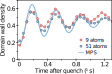
\includegraphics[height=3cm]{img/2_projet_recherche/scars_DW_density}
		
		Expérience : blocage de Rydberg
		
		\footnotesize{[Bernien \emph{et al} 17]}
	\end{column}
\end{columns}
\begin{block}{\textbf{Projet} [Anna Minguzzi, Robert Whitney]}
	\begin{itemize}
		\item Conditions d'existence ?
		\item Couplage à l'environnement ?
	\end{itemize}
\end{block}
\end{frame}

\begin{frame}{Circuits quantiques}
\begin{enumerate}
	\item Structure simple $\to$ description \textbf{exacte}
	\item Hydrodynamique (grands $t$ et $x$) $\to$ description \textbf{universelle}
\end{enumerate}
\begin{columns}
	\begin{column}{0.5\textwidth}
		\centering
		\includegraphics[height=3cm]{img/2_projet_recherche/circuit}
				
		\footnotesize{[Chan, De Luca, Chalker 18]}
	\end{column}
	\begin{column}{0.6\textwidth}
		\begin{block}{\textbf{Projet} \footnotesize{[L.\ Canet, V.\ Rossetto, C.\ Branciard, P.\ Arrighi]}}
			\begin{itemize}
				\item Systèmes critiques ?
				\item Désordre ? 2D ?
				\item Dynamique de l'information et efficacité des algorithmes quantiques ?
			\end{itemize}
		\end{block}
		\begin{block}{\textbf{Expertise numérique}}
			Diagonalisation exacte innovante
		\end{block}
	\end{column}
\end{columns}
\end{frame}

\section{Activités d'enseignement}
\subsection{Dummy}
\begin{frame}{Actions collectives}
\begin{columns}
\begin{column}{0.6\textwidth}
\begin{block}{Responsabilités collectives}
\begin{itemize}
	\item Organisation des rencontres des jeunes physicien$\cdot$ne$\cdot$s
\end{itemize}
\end{block}
\begin{block}{Médiation \& vulgarisation scientifique}
\begin{itemize}
	\item Animation (Fête de la Science, Pint of Science)
	\item Ma thèse en 180 secondes
	\item Supports scientifiques (articles, vidéo)
\end{itemize}
\end{block}
\end{column}
\begin{column}{0.4\textwidth}
\centering
\includegraphics[width=\columnwidth]{img/3_projet_enseignement/fete_de_la_science}
\end{column}
\end{columns}
\end{frame}

\begin{frame}{Enseignement}
\begin{itemize}
	\item Tutorat de maths - L1 $\sim$ 20 h
	\item Optique géométrique (cours, TD, TP) - L1 $\sim$ 20 h
	\item Mécanique du solide \& physique des ondes (TD et TP) - L2 $\sim$ 160 h
	\item \textbf{Projet professionnel} - L1 $\sim$ 27 h
\end{itemize}
\end{frame}

\section{Projet d'enseignement}
\subsection{Dummy}
\begin{frame}{Séquence d'enseignement : Phénomènes ondulatoires -- L2, 60 heures}
Plan de cours :
\begin{columns}
	\begin{column}{0.5\textwidth}
		\begin{block}{\textbf{Ondes dans les milieux}}
			\begin{enumerate}
				\item Rappels : oscillateurs mécaniques,
				\item Cordes, ondes progressives,
				\item Ondes sonores, impédance,
				\item Ondes stationnaires, résonance.
			\end{enumerate}
		\end{block}
	\end{column}
	\begin{column}{0.5\textwidth}
		\begin{block}{\textbf{Optique ondulatoire}}
			\begin{enumerate}
				\item Ondes lumineuses,
				\item Interférences à deux ondes,
				\item Interférences à $N$ ondes,
				\item Polarisation.
			\end{enumerate}
		\end{block}
	\end{column}
\end{columns}
\begin{block}{\textbf{Défis}}
	\begin{itemize}
		\item Universalité des phénomènes ondulatoires $\to$ prise de recul
		\item Ondes lumineuses : évasives
	\end{itemize}
\end{block}
\end{frame}

\begin{frame}{La séquence en pratique}
\begin{block}{Fonctionnement en \textbf{classe inversée} :}
\begin{enumerate}
	\item \textbf{À la maison} ($\sim$ 4 h) : cours, exercices de compréhension (correction en ligne),
	\item \textbf{Cours} ($\sim$ 2 h) : applications directes, discussions,
	\item \textbf{TD} ($\sim$ 2 h) : travail d'approfondissement \textbf{en groupe},
	\item \textbf{TP} : 4 h, certaines semaines.
\end{enumerate}
\end{block}
\end{frame}

\begin{frame}{Une unité : Introduction aux interférences à deux ondes}
\begin{itemize}
	\item \textbf{À la maison} : conditions des interférences, interférences constructives/destructives, franges, etc.
	\item \textbf{En classe} : deux ondes planes, manip : cuve à ondes.
	\item \textbf{TD numérique} : deux ondes cylindriques.
\end{itemize}
\centering
\includegraphics[width=0.4\columnwidth]{img/3_projet_enseignement/interf_cylindriques}
\end{frame}

\begin{frame}{Bonus : vulgarisation en L1-L2}
Inspiration : UE \emph{Culture biologie numérique} à l'Université Paris Diderot.

Vulgarisation d'un thème de L1-L2 via un \textbf{article de blog} et un oral (cf ``physics show'' d'Orsay).

\begin{columns}
\begin{column}{0.6\textwidth}
\begin{block}{Objectifs :}
	\begin{itemize}
		\item Réappropriation des notions,
		\item Travail en groupe,
		\item Projet,
		\item Découverte de la vulgarisation.
	\end{itemize}
\end{block}
\end{column}
\begin{column}{0.4\textwidth}
\centering
\includegraphics[width=\columnwidth]{img/3_projet_enseignement/banniere-cafe-big6}
\end{column}
\end{columns}
\end{frame}
\section{Conclusion}
\subsection{Dummy}
\begin{frame}{Conclusion}

\begin{columns}
	\begin{column}{0.4\textwidth}
		Travaux
			\begin{itemize}
				\item Quasipériodicité
				\item Localisation à $N$ corps
				\item Circuits quantiques
			\end{itemize}
		\end{column}
		\begin{column}{0.2\textwidth}
			$\xrightarrow[\text{Physique à $N$ corps}]{\text{méthodes numériques}}$
		\end{column}
		\begin{column}{0.4\textwidth}
			\textbf{Recherche au LPMMC}
			\begin{itemize}
				\item Cohérence quantique (localisation à $N$ corps, états non-ergodiques)
				\item Couplage à environnement et thermalisation (dynamique de l'information quantique)
			\end{itemize}
			
			\begin{block}{\textbf{Enseignement à l'UGA}}
	\begin{itemize}
		\item Suivi, orientation
		\item Pédagogies actives
		\item Enseignement par projets
	\end{itemize}
\end{block}

		\end{column}
	\end{columns}
\end{frame}

\section{Questions}
%Each section needs a subsection for the small points on top to show up
\subsection{Dummy}

\begin{frame}{Multifractalité de la chaîne de Fibonacci}
Invariance d'échelle géométrique $\implies$ multifractalité du spectre et des fonctions d'onde

\centering
\includegraphics[width=0.5\columnwidth]{img/4_questions/recursive_construction_spectrum}
\end{frame}

\begin{frame}{Multifractalité de la phase localisée à $N$ corps}

\centering
\includegraphics[width=0.4\columnwidth]{img/4_questions/scalings}
%
\includegraphics[width=0.4\columnwidth]{img/4_questions/scaling-laws-Fock}

\end{frame}

\begin{frame}{Multifractalité et transitions de phase}
\centering
\includegraphics[width=0.6\textwidth]{img/4_questions/Dq}
\end{frame}

\begin{frame}{Blocage de Rydberg et dynamique contrainte}
Nombre quantique principal élevé ($n \geq 50$) $\to$ interactions fortes

Deux atomes :
\[
	H = \Omega( X_1 + X_2) + V Q_1 Q_2
\]
$Q = \frac{1 + Z}{2}$, Van der Waals : $V \propto 1/r^6$.

Régime de blocage de Rydberg : $V \gg \Omega$ $\to \xcancel{\uparrow \uparrow}$
\end{frame}

\begin{frame}{Diagonalisation exacte des circuits quantiques}
Circuits de \textbf{Floquet} : opérateur d'évolution périodique de période $\tau$:
\[
	\ket{\psi(t = n \tau)} = U^n \ket{\psi(0)}
\]
$U$ \textbf{matrice dense} $2^L \times 2^L$ $\implies$ stockage impossible pour $L > 15$.

Circuit quantique 

$\implies$ $U = $ \textbf{opérateur produit de matrices} (MPO) 

$\implies$ opération $y = U x$ rapide et parallélisable en ``matrix free''

$\implies$ diagonalisation exacte (méthode itérative) jusqu'à $L = 20$.

\end{frame}

\begin{frame}{Description hydrodynamique de l'information quantique}
\begin{block}{Modèle microscopique : croissance d'interface}
\centering
\includegraphics[width=0.4\columnwidth]{img/4_questions/applyingUnitary}

\footnotesize{[Nahum \emph{et al} 17]}
\end{block}
Régime hydrodynamique : KPZ
\[
	\frac{\partial S}{\partial t} = \nu \partial_x^2 S - \frac{\lambda}{2} (\partial_x S)^2 + \eta(x,t) + c
\]

Universalité : exacte pour entropie de Hartley, $d \to \infty$, conjecture : unitaires aléatoires, unitaires de Clifford, chaîne XXZ + environnement \footnotesize{[Nahum \emph{et al} 17, Knap 18]}.
\end{frame}

\begin{frame}{Simulations dans le formalisme de Lindblad}
Flot de Lindblad 
\[
	\frac{d \rho}{d t} = i[\rho, H] + \gamma \sum_k\left( [L_k \rho, L_k^\dagger] + \text{h.c} \right)
\]
Algorithme : 
\begin{enumerate}
	\item Représentation MPO de $\rho$ (troncature éventuelle)
	\item Action du Liouvillien décomposé (Trotter-Suzuki)
\end{enumerate}
Facteur limitant : entropie d'opérateur bornée. Simulation de l'ordre de 100 spins ou qubits.
\end{frame}

\begin{frame}{Atomes froids quasipériodiques}
\centering
\includegraphics[width=0.5\columnwidth]{img/4_questions/cold_atoms_qc}
\end{frame}

\begin{frame}{Machines thermiques MBL}
Cycle à 4 temps quantique

\begin{columns}
\begin{column}{0.5\textwidth}
\centering
\includegraphics[width=0.8\columnwidth]{img/4_questions/Otto_cycle_MBL}

\footnotesize{[Halpern 18]}
\end{column}
\begin{column}{0.5\textwidth}
\begin{align*}
	\mathcal{P}_v^\text{voiture} &= 1~\text{MW}/\text{m}^3 \\
	\mathcal{P}_v^\text{MBL} &= 100~\text{kW}/\text{m}^3 \\
	\mathcal{P}_v^\text{boîte quantique} &= 1~\text{kW}/\text{m}^3 \\
\end{align*}
\end{column}
\end{columns}
\end{frame}

\begin{frame}{Fidelité et dimensions fractales}
\[
	F(t) = |\braket{\psi(0)}{\psi(t)}|^2
\]
Partant d'un état polarisé en spin,
\[
	F(t\to\infty) = e^{-S_2} = \mathcal{N}^{-D_2}
\]
Imbalance finale d'un état polarisé en spin $\mathcal{C}_0$ :
\[
	I(t \to \infty) = \sum_{k,\mathcal{C}} |\braket{k}{\mathcal{C}}|^2 |\braket{k}{\mathcal{C}_0}|^2 \delta(\mathcal{C}_0, \mathcal{C})
\]
où $-1 \leq \delta(\mathcal{C}_0, \mathcal{C}) \leq 1$ mesure la distance entre les deux configurations.
\end{frame}

\begin{frame}{Bicouches de graphène quasipériodiques}
\centering
\includegraphics[width=0.5\columnwidth]{img/4_questions/QC_bilayer}

[Yao \emph{et al} 18]
\end{frame}

\begin{frame}{Circuit quantique critique}
\begin{columns}
\begin{column}{0.5\textwidth}
\centering
\includegraphics[width=\columnwidth]{img/4_questions/rgaps}
\end{column}
\begin{column}{0.5\textwidth}
\centering
\includegraphics[width=\columnwidth]{img/4_questions/OpEnt_bottlenecks}
\end{column}
\end{columns}
\end{frame}



\end{document}